%THIS SECTION IS TO DESCRIBE THE SYSTEM ARCHITECTURE AND HOW IT WORKS (MORE ABOUT IMPLEMENTATION)
\section{PrAd}

%In this section, we describe an architecture of \codename. We give details on how our model can serve LBA without compromising users' location privacy. Finally we suggest an accounting procedure.

\subsection{Architecture}
\codename proposes two changes to the traditional LBA architecture. As displayed in figure \ref{fig:architecture}, the first component of \codename is a small service called $mPrAd$ running in user's smartphone. Unlike traditional model of LBA where ads-funded mobile applications establish connections and retrieve ads directly from $LBAS$, in our model, they just need to call $mPrAd$ service.
This small service serves as a client in our model to perform private ads retrieval, and then forwards retrieved ads to ads-funded application. 
It also be responsible in constructing billing vector in homomorphic encryption form and send it to $LBAS$. $mPrAd$ contains two secret key, one for performing space-encoding and the other one is to encrypt billing vector. The reason to delegate these tasks to a small independent service like $mPrAd$ is that ads-funded applications are not always trusted. There are incentives for such ads to leak user's sensitive information. Mobile applications can be designed to look benevolent to pass vetting procedure of apps publisher but become malicious once it is installed on user's phone \cite{jekyll}. Hence, it is not necessary for ads-funded application to access location sensor, which is required in the first place for space-encoding process, unless there is an explicit need of location information to facilitate its authorized activities. The other reason is that there are so many apps developers that distributing a set of secret keys required in our model incurs many complications. By introducing $mPrAd$, we can avoid such secret key distribution problem. One more reason is that there may be so many ads-funded application running in the same smartphone; and running a single $mPrAd$ to serve all of those ads can save computational and communication cost compared to each application perform ads retrieval separately. The second change involves the presence of a trusted secure processor. Specifically, SC is required to be installed on $LBAS$ and every request to $LBAS$ is routed through this SC. Note that this SC is able to read and write data to $LBAS$'s database.



% a figure is very good way to demmostrate
\begin{figure}*
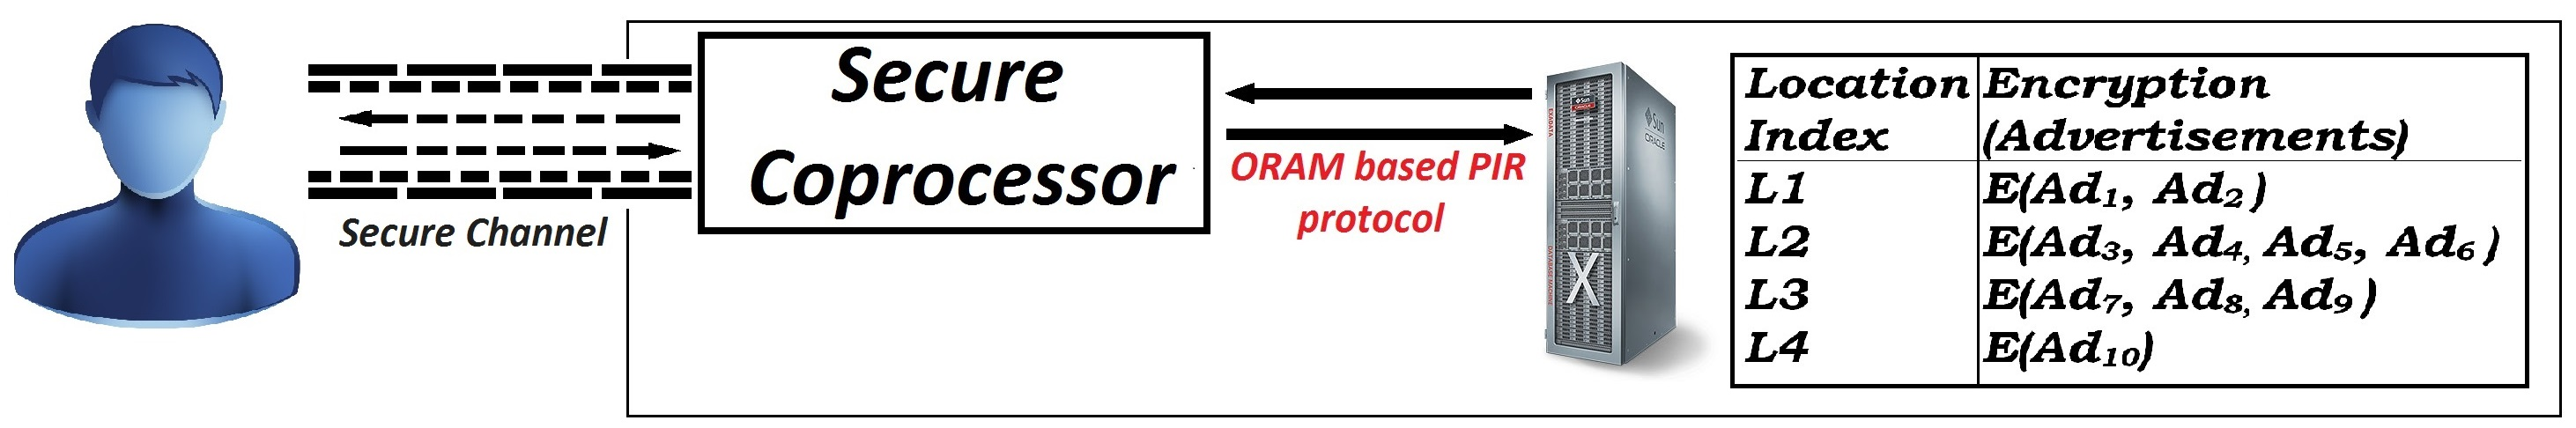
\includegraphics[scale=0.3]{figures/architecture_img.jpg}
\caption{\codename architecture}
\label{fig:architecture}
\end{figure}




\subsection{How \codename works}
% talk about the workflow here.
We assume that there are many ads co-locating at the same area. For example, there are many products from different brands offered in one supermarket, and all these brands want to launch LBA services for their products. \codename groups all ads that are in the same are into one set, in indexes such a set with the space-encoded value of that area. Without loss of generality, we assume that there is a square bounding the entire region. Then, we divide such square into $x$ units where $x$ is a square number. Each square unit is represented by its mid-point. Our approach use the space-encoding technique proposed in \cite{Space_Transformation} to calculate Hilbert values of all those points and use those values to index corresponding square unit. Thus, the ads database of \codename will comprises of records of form \textit{<Index - set of Ads>}. It follows that there will be squares unit containing ads and some others don't. \codename only keeps track of those square that unit that contains ads and doesn't index empty square in its database. Note that besides all ads submitted by Advertisers, \codename stores a special ads record whose index is $Defaul\ Index$ which is served to users who have no ads in their proximity.


In order to initialize $LBAS$, the SC follows the offline preprocess phase of the protocol discussed in subsection \ref{subsec:PIR}. After the initialization phase finishes, $LBAS$ is ready to server LBA service.
When an ads-funded mobile application is in use, it call the $mPrAd$ service to retrieve ads. $mPrAd$ first collects exact location information from sensor (i.e. GPS sensor) and perform the space-encoding. It then establishes a secure channel to SC, encrypts the request with SC's public key and submit it. The SC receives the encrypted request, decrypt it using its private key, and perform a private ads retrieval detailed in Algorithm 1. The SC then encrypts the ads with $mPrad$'s public key and sends it back to $mPrAd$. Upon receiving response from SC, $mPrAd$ decrypts the response and forward a set of ads to mobile applications. For every ads displayed, the application send an acknowledge to $mPrAd$. Based on these acknowledges, $mPrAd$ can keep counters of how many times each ads is displayed. At the end of a billing period, $mPrAd$ build a billing vector, encrypts it and sends it to $LBAS$, follow the procedure outlined in subsection \ref{subsec:billing}.

Recall that our space encoder utilizes space-filling curve, which reserves neighborhood and locality of spatial data object; i.e. if two spatial object are near each other, their spatial indices calculated by our space encoder will also very close to each other. Because of this interesting property, our framework allows extra flexibility in serving ads. Specifically, users can decide on a range of the area in which they want to retrieve ads. Based on user's settings, $mPrAd$ can send more than one requests to $LBAS$ to retrieve ads in a wider area. Despite sending more than one requests, $mPrAd$ only needs to calculate one index, with is a space-encoded index of user's current location; then it send requests with consecutive indices of the calculated one. For example, if the user opts to retrieve ads in an area that is 3 times larger than default square unit, and her current location's index is $l$, then $mPrAd$ will sends 3 requests with indices $l$-1, $l$, $l$+1 to $LBAS$.




\subsection{Security}
We claim that \codename can obtain strong location privacy. We justify this claim by sequentially proving that in delivering ads to users, \codename satisfies all three security metrics discussed in section \ref{sec:background}. In addition, the use of homomorphic encryption and k-anonymity concept in \codename 's billing procedure further fortifies our claim.

Given the presences of SC, there is no direct interaction between users and LBAS. The only interaction between LBAS and SC is facilitated through the private retrieval detailed in Algorithm 1. That is, in the view of the LBAS, every request is exactly the same as each other no matter by whom it is issued. Thus, our technique satisfy the \textit{u-anonymity} metric.
Thanks to the space encoding as well as the double-encryption and database permutation privately performed in each ads retrieval, LBAS cannot figure out which POI is actually received interest. That is, it doesn't know from where user sent their request. Thus, \textit{a-anonymity} is guaranteed. 
Finally, as described in Algorithm 1, with respect to the view of LBAS, the SC performs exactly the same sequence of operations and (permuted) database access for every ads retrieval. Specifically, it reads one accessed record and one unaccessed record to its memory $M$, and then replace those two records with randomly chosen and doubly encrypted item from $M$. Thus, we argue that our ads retrieval approach is \textit{data-oblivious}, which nullifies LBAS's ability of carrying out inference or correlation attack based on database's access frequency. It is clear that our technique appreciates all three privacy metrics, \textit{a-anonymity}, \textit{u-anonymity}, and \textit{data-oblivious execution}; hence, it follows that our technique achieves strong location privacy in ads retrieval. In billing process, ads-reports are collected anonymously so that LBAS cannot learn which ads is displayed on which user's app. 

